\chapter{Diffusion Models}

\ca{Asegurarme la consistencia de notación con $\mathrm{x}$ y no $x$.}

\begin{figure}[ht]
    \centering
    \includegraphics[scale=0.22]{ch2-diffusion-models/fwd_noise.png}
    \captionsetup{width=\textwidth} % set the width of the caption
    \caption{Grogu (aka baby Yoda) through a forward process...\ca{Ver como mejorar estas imagen en resolución...}}
    \label{fig:fwd-process-grogu}
\end{figure}
  
In this chapter, we introduce the Diffusion Model, a family of generative models that have proven to be a valuable framework for model novel image generation artefacts, such as Dall-E (\ca{Agregar más aplicaciones y referencias particulares, basarse en algún survey como el de Yan Song}) and Stable Diffusion and have provided active research lines in the last few years.\\

We will review the formulation proposed in the work titled \textit{Denoising Diffusion Probabilistic Models} \cite{ho2020denoising}, or DDPM for short. The primary motivation to base the discussion about Diffusion Models from this work is that it serves as a framework to understand the following improvements and enhancements without much modifications from the primary ingredients of the recipe. Moreover, it has a deep connection with Score-based models \cite{song2020denoising} and can be understood as Hierarchical Variational Autoencoders as explained in the \cite{luo2022understanding}.\\

\section{Model}

From DDPO: "The key idea behind diffusion models is to iteratively transform a simple prior distribution into a target distribution by applying a sequential denoising process".

In DDPM, there is a forward process which starts from the raw image (or input) $\mathbf{x}_{0}$ and creates a sequence
of intermediate steps between $\mathbf{x}_{1}$ and $\mathbf{x}_{T-1}$, also known as latent states, that are noise perturbations in some degree of the original image's structure.\\ 

At the end of the sequence $T$, the image is ultimately converting into an isotropic Gaussian noise $\mathbf{x}_{T}\sim \mathcal{N}(\mathbf{0}, \sigma^2\mathbf{I})$\footnote{Isotropic is a fancy word for "equal shape", and in this context means that the direction of the covariance matrix is all equal.}.\\

The authors model this forward process $q(\mathbf{x_{1:T}}\mid\mathbf{x}_{0})$ as a Markov chain, and it
is follow a normal distribution without learnable 
parameters.
\begin{align}
q(\mathbf{x}_{1:T}\mid\mathbf{x}_0) = \prod_{t=1}^{T}q(\mathbf{x}_t\mid\mathbf{x}_{t-1})
\\
q(\mathbf{x}_t\mid\mathbf{x}_{t-1}) = \mathcal{N}(\mathbf{x}_t;\sqrt{1-\beta_{t}}~\mathbf{x}_{t-1},~ \beta_{t}\mathbf{I})
\end{align}

At the same time, parallel to the forward process, there is
a backward process, model by $p_{\theta}(\mathbf{x}_{T:0})$.\\

A deterministic linear noise scheduler is known beforehand and gives us for any $t$ the right amount of noise $\beta_{t}$ to generate $\mathbf{x}_{t}$. \\

How do we think about the latent space? The scale-location transformation\footnote{A quick recap about normal distributions, if $Z$ is a standard normal random variable and $X=\mu + \sigma Z$, then $X$ is a normal random variable with mean $\mu$ and
variance $\sigma^2$, i.e. $X\sim\mathcal{N}(\mu, \sigma^2)$.
Keep that in your mind.} of $q(x_{t}~|x_{t-1})\sim\mathcal{N}(x_{t}; \sqrt{1-\beta_{t}} x_{t-1}, \beta_{t}\mathbf{I})$ allow us sample the \textcolor{orange}{current latent state $x_{t}$ as a mixture} of \textcolor{violet}{how
much perturbation inject} from nose $\epsilon_{t-1}$, and \textcolor{teal}{the rest of what left of the image's structure} from the previous latent space $x_{t-1}:$

$$
\textcolor{orange}{x_{t}} = \textcolor{teal}{\sqrt{1-\beta_{t}}} x_{t-1} + \textcolor{violet}{\sqrt{\beta_{t}}}\epsilon_{t-1}
$$

\section{Recursive Reparameterization Trick}

The reparameterization trick originally appears in the work that introduce the Variational Autoencoder model \cite{kingma2013auto} and is used as well in the diffusion framework with minor modifications. The main goal is removing the stochasticity of a node variable---that depends on parameters from the distribution. As simple it appears, that makes possible to backpropagate properly, and update the parameters during training. \\

Let $\alpha_{t}=1 - \beta_{t}$ and $\bar{\alpha}_{t}=\prod_{i=1}^{t}\alpha_{i}$. Now we proceed
to unwind the $t$ index until $t=0$ in the sampling formula
that we can sample from any arbitrary normal distribution just
scaling the normal standard distribution $\sim \mathcal{N}(0, \sigma^2)$ accordingly its parameters:
\begin{equation}\label{reparameterization-trick}
    \begin{split}
            x_{t} & = \sqrt{\alpha_{t}}~x_{t-1} + \sqrt{1-\alpha_{t}}~\epsilon_{t-1} \\
             & = \sqrt{\alpha_{t}}~(\sqrt{\alpha_{t-1}}~x_{t-2} + \sqrt{1 - \alpha_{t-1}}~\epsilon_{t-2}) + \sqrt{1-\alpha_{t}}~\epsilon_{t-1} \\
             &= \sqrt{\alpha_{t}~\alpha_{t-1}}~x_{t-2} + \textcolor{teal}{\sqrt{\alpha_{t} - \alpha_{t}~\alpha_{t-1}}~\epsilon_{t-2} + \sqrt{1-\alpha_{t}}~\epsilon_{t-1}} \\
             & = \sqrt{\alpha_{t}~\alpha_{t-1}}~x_{t-2} + \textcolor{teal}{\sqrt{1 - \alpha_{t}~\alpha_{t-1}}~\bar{\epsilon}_{t-2}} \\
             & = \dots \\
             & = \sqrt{\alpha_{t}~\alpha_{t-1}\dots\alpha_{0}}~x_{0} + \sqrt{1 - \alpha_{t}~\alpha_{t-1}\dots\alpha_{0}}~\epsilon \\
             &= \sqrt{\bar{\alpha}}~x_{0} + \sqrt{1 - \bar{\alpha}}~\epsilon \\
            q(x_{t}\mid x_{0}) & = \mathcal{N}(x_{t};\sqrt{\bar{\alpha}_{t}}~x_{0}, (1-\bar{\alpha}_{t})~\mathbf{I})
    \end{split}
\end{equation}

The remarkable consequence of the reparameterization trick is that
we have a closed form to sample from $x_{0}\rightarrow x_{t}$
without passing explicitly for intermediate steps $x_{1}, \dots, x_{t-1}$. Therefore, we can go from $x_{0}$ to
any arbitrary $t$ in just one evaluation, making the whole DDPM framework computationally feasible.


\section{Optimization}

\subsection{Variational Lower Bound}

    DDPM are training by optimizing the variational lower bound
    on the negative log-likelihood.
    
    \begin{equation}\label{eqn:ELBO1}
    \begin{split} 
    \mathop{\mathbb{E}}[-\log p_{\theta}(x_{0})] & \leq \mathbb{E}_{q}\bigg[-\log \frac{p_{\theta}(x_{0:T})}{q(x_{1:T}|~x_{0})}\bigg] \\
    & \leq \mathbb{E}_{q}\bigg[-\log p(x_{T}) - \sum_{t\geq 1}^{T} \log\frac{p_{\theta}(x_{t-1}|~x_{t})}{q(x_{t}|~x_{t-1})} \bigg] \\
    L & := \mathbb{E}_{q}\bigg[-\log p(x_{T}) - \sum_{t>1}^{T} \log \frac{p_{\theta}(x_{t-1}|~x_{t})}{q(x_{t}|~x_{t-1})}-\log\frac{p_{\theta}(x_{0}|~x_{1})}{q(x_{1}|~x_{0})}\bigg]
    \end{split}
    \end{equation}
    
    Recall that the Markovian property is applied to the forward
    and backward processes. This explains the step 2 in the above
    Eq.~\ref{eqn:ELBO1}. Also, notice that we decouple the last term $x_{T}$ from the $p_{\theta}(x_{0:T})$ because
    for a sufficiently large sequence $T\gg$ we know that we will get a final state described by a $\mathcal{N}(\mathbf{0}, \sigma^2\mathbf{I})$, so we keep separate in the same way
    that the first transition step that involves the raw image $x_{0}$. \\
    
    Therefore, the following derivations in \cite{ho2020denoising}
    and \cite{sohldickstein2015deep} we obtain the training objective from the Variational Lower Bound (VLB):

    \begin{equation}\label{eqn:ELBO2}
    \begin{split}
    L & = \mathbb{E}_{q}\bigg[-\log p(x_{T}) - \sum_{t>1}^{T} \log \frac{p_{\theta}(x_{t-1}|~x_{t})}{q(x_{t}|~x_{t-1})}-\log\frac{p_{\theta}(x_{0}|~x_{1})}{q(x_{1}|~x_{0})}\bigg] \\
    & = \mathbb{E}_{q}\bigg[-\log p(x_{T}) - \sum_{t>1}^{T} \log \frac{p_{\theta}(x_{t-1}|~x_{t})}{\textcolor{teal}{q(x_{t-1}|~x_{t}, x_{0})}}\frac{\textcolor{lightgray}{q(x_{t-1}|~x_{0})}}{\textcolor{violet}{q(x_{t}|~x_{0})}}-\log\frac{p_{\theta}(x_{0}|~x_{1})}{q(x_{1}|~x_{0})}\bigg] \\
    & = \mathbb{E}_{q}\bigg[-\log p(x_{T}) - \sum_{t>1}^{T} \log \frac{p_{\theta}(x_{t-1}|~x_{t})}{\textcolor{teal}{q(x_{t-1}|~x_{t}, x_{0})}} -\sum_{t>1}^{T}\log \frac{\textcolor{lightgray}{q(x_{t-1}|~x_{0})}}{\textcolor{violet}{q(x_{t}|~x_{0})}}-\log\frac{p_{\theta}(x_{0}|~x_{1})}{q(x_{1}|~x_{0})}\bigg] \\
    & = \mathbb{E}_{q}\bigg[-\log p(x_{T}) - \sum_{t>1}^{T} \log \frac{p_{\theta}(x_{t-1}|~x_{t})}{\textcolor{teal}{q(x_{t-1}|~x_{t}, x_{0})}}- \log\frac{\textcolor{orange}{q(x_{1}|~x_{0})}}{\textcolor{violet}{q(x_{T}|~x_{0})}} -\log\frac{p_{\theta}(x_{0}|~x_{1})}{q(x_{1}|~x_{0})}\bigg] \\
    & = \mathbb{E}_{q}\bigg[-\log p(x_{T}) - \sum_{t>1}^{T} \log \frac{p_{\theta}(x_{t-1}|~x_{t})}{\textcolor{teal}{q(x_{t-1}|~x_{t}, x_{0})}}- \log\textcolor{orange}{q(x_{1}|~x_{0})} + \log \textcolor{violet}{q(x_{T}|~x_{0})} -\log\frac{p_{\theta}(x_{0}|~x_{1})}{q(x_{1}|~x_{0})}\bigg] \\
    & = \mathbb{E}_{q}\bigg[-\big(\log p(x_{T}) - \log \textcolor{violet}{q(x_{T}|~x_{0})}\big) - \sum_{t>1}^{T} \log \frac{p_{\theta}(x_{t-1}|~x_{t})}{\textcolor{teal}{q(x_{t-1}|~x_{t}, x_{0})}} - \big( \log\textcolor{orange}{q(x_{1}|~x_{0})}  +\log\frac{p_{\theta}(x_{0}|~x_{1})}{q(x_{1}|~x_{0})}\big)\bigg]  \\ 
    & = \mathbb{E}_{q}\bigg[-\log \frac{p(x_{T})}{\textcolor{violet}{q(x_{T}|~x_{0})}} - \sum_{t>1}^{T} \log \frac{p_{\theta}(x_{t-1}|~x_{t})}{\textcolor{teal}{q(x_{t-1}|~x_{t}, x_{0})}} -  \log p_{\theta}(x_{0}|~x_{1})\bigg]  \\
    & L_{\text{\scriptsize{\text{VLB}}}}= \mathbb{E}_{q}\bigg[\underbrace{D_{\text{\scriptsize{KL}}}\big(\textcolor{violet}{q(x_{T}|~x_{0})} ||~p(x_{T}) \big)}_{L_{T}} + \sum_{t>1}^{T} \underbrace{D_{\text{\scriptsize{KL}}}\big( \textcolor{teal}{q(x_{t-1}|~x_{t}, x_{0})}||~p_{\theta}(x_{t-1}|~x_{t}) \big)}_{L_{t-1}} -  \underbrace{\log p_{\theta}(x_{0}|~x_{1})}_{L_{0}} \bigg]
    \end{split}
    \end{equation}
    
    We notice three kinds of terms in Eq.~\ref{eqn:ELBO2}

\subsection{Denoising Matching Term}

\textbf{TODO:} Mejorar esta parte...

The model goal is to reduce the discrepancy measured by the $(D_{KL})$ between both distributions, the posterior of the encoder, which added the noise, and the decoder, which predicts to "reverse" the processes and has learnable parameters $(\theta)$. Therefore, the loss constitutes a sum of denoising matching terms across the diffusion sequence.

\begin{figure}[ht]
  \centering
  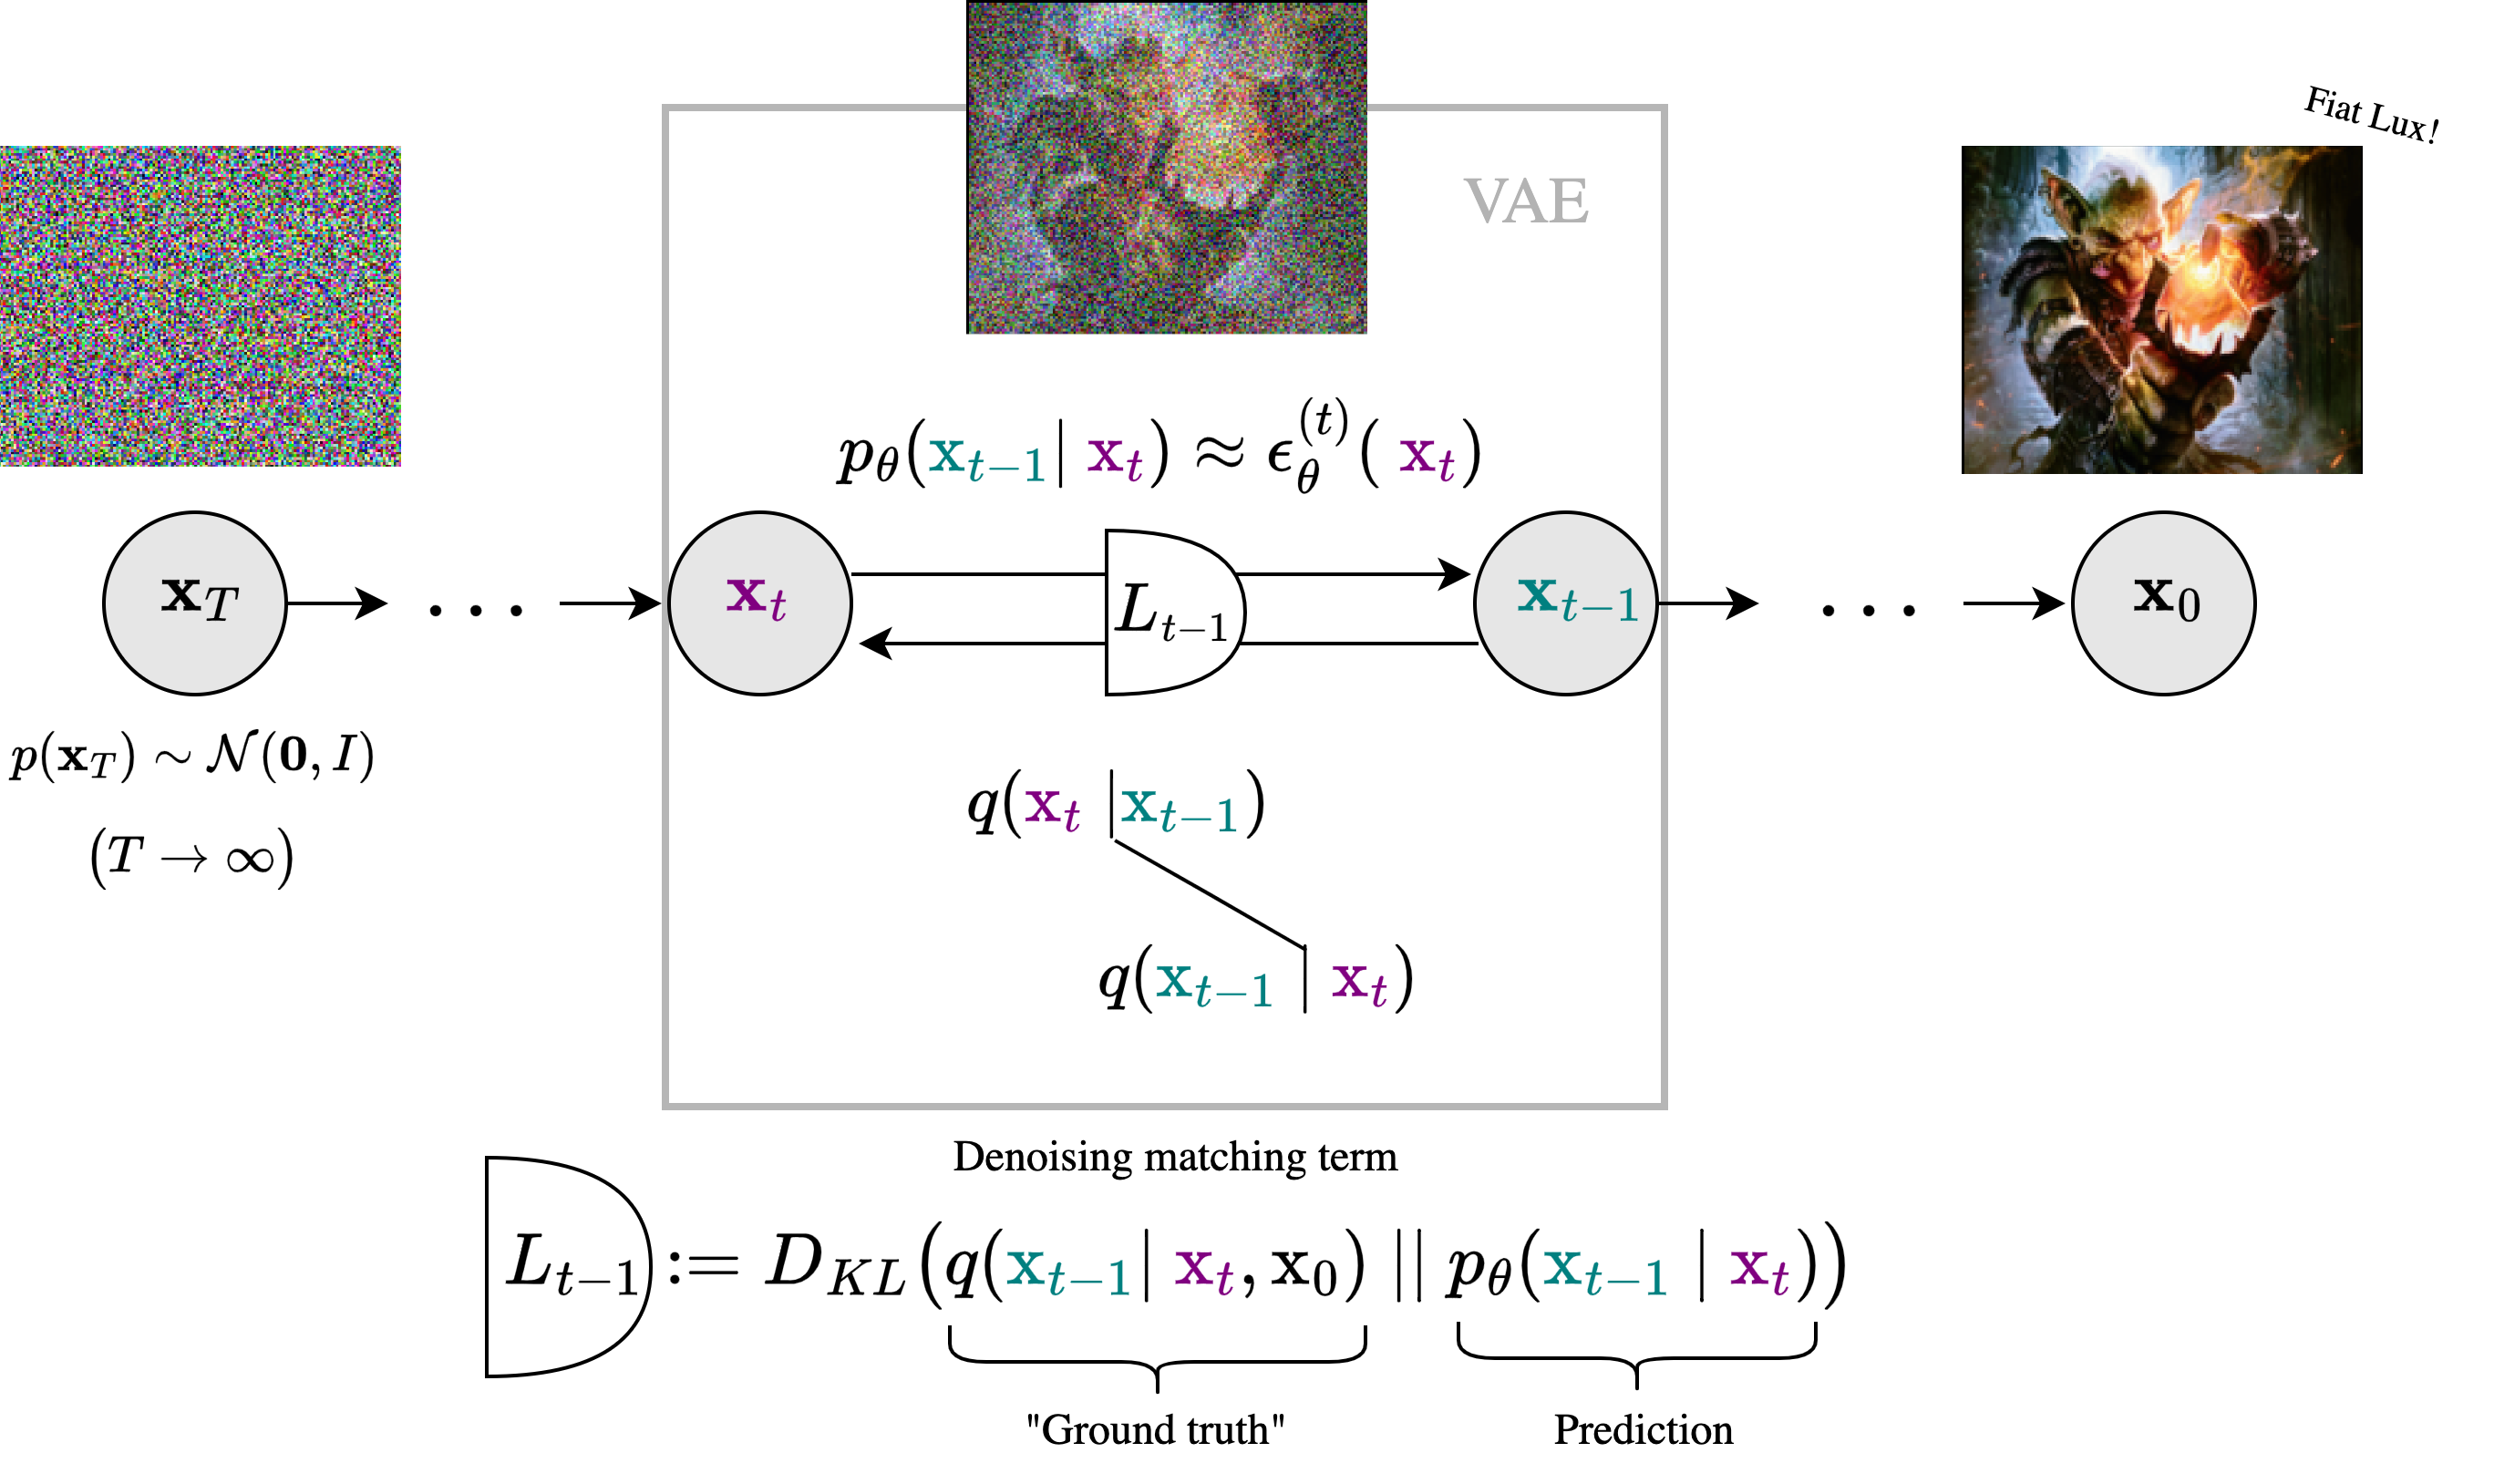
\includegraphics[scale=0.8]{ch2-diffusion-models/DDPM-HMVAE-simple.png}
  \captionsetup{width=\textwidth} % set the width of the caption
  \caption{\textbf{Denoising matching term in action.} $\mathrm{x}_{T}$ is a pure Gaussian noise. In the middle square, it highlights the transition from a noisy intermediate state to a less noisy one; the denoising matching term forces $p_{\theta}$ to be similar to the posterior forward kernel $q(\mathrm{x}_{t-1}\mid \mathrm{x}_{t})$. $\mathrm{x}_{0}$ the input image during training or the final sample at inference mode. \ca{Simplicar este caption esta muy verboso.}}
  \label{fig:ddpm-denoising-term}
\end{figure}

\textbf{TODO}: In Fig.~\ref{fig:ddpm-denoising-term}, we conditioned $q$ on $x_{0}$ to make tractable. Write more details about this...\\

\textbf{TODO}: Derived the closed expression between two Gaussian KL.
    
\section{Condition the model}

So far, we know how to learn indirectly the unconditional probability distribution $p(x)$ via the score function $\nabla_{x}\log p(x)$, but what can we do to condition $x$ given a signal $y$, such as a text prompt, another image, or an audio?\\

By Bayes' theorem, log operations, and taking the gradient w.r.t. x we got:

    \begin{equation}
         \begin{split}
            p(x \mid y) &= \frac{p(y \mid x) \cdot p(x)}{p(y)}\\
            \implies \log p(x \mid y) &= \log p(y \mid x) + \log p(x) - \log p(y) \\
            \implies \nabla_x \log p(x \mid y) &= \nabla_x \log p(y \mid x) + \nabla_x \log p(x) ,
        \end{split}
    \end{equation}
    

    \textbf{TODO:} Review and cite the following \href{https://sander.ai/2023/08/28/geometry.html}{blog posts} \cite{dieleman2022guidance} and \cite{dieleman2023geometry} about guidance.

\subsection{Classifier Guidance}

    Once a diffusion model is trained, during the sampling
    process (aka denoising Gaussian noise), we can attach
    a cost function that "guides" the denoising process toward
    some desired condition, such as colour or text embedding from a prompt that matches a text caption, gets by the image at each denoising step.\\ Introduce in \cite{nichol2021glide}.

    \textbf{TODO:} Mention and explain the Relevant work in the last part of this work \cite{Dhariwal2021DiffusionMB}.\\     

    \ca{\textbf{TODO:} Agregar ejemplos de classifier guidance con las caras.\\}

    \textbf{TODO:} Create a diagram to explain the classifier guidance. It could be used for text prompt guidance using CLIP.\\ \ca{Lo importante es mencionar como usar el espacio de embedding conjunto de CLIP en los modelos text-to-image para guairlos...}.
    
\subsection{Classifier Free Guidance}

    \textbf{TODO:} A good blog post that explains classifier guidance is \cite{dieleman2022guidance}. \\


\section{Enhancements \& Improvements}

Despite the progress in conditioning the model, there are...\\

A direct improvement to the DDPM was made in \cite{nichol2021improved}, in which they learn not only $\mu$ but also the variance $\sigma^{2}$ of the reverse process. This directly improves the likelihood estimation achieved by the model. \\

\begin{figure}[ht]
    \centering
    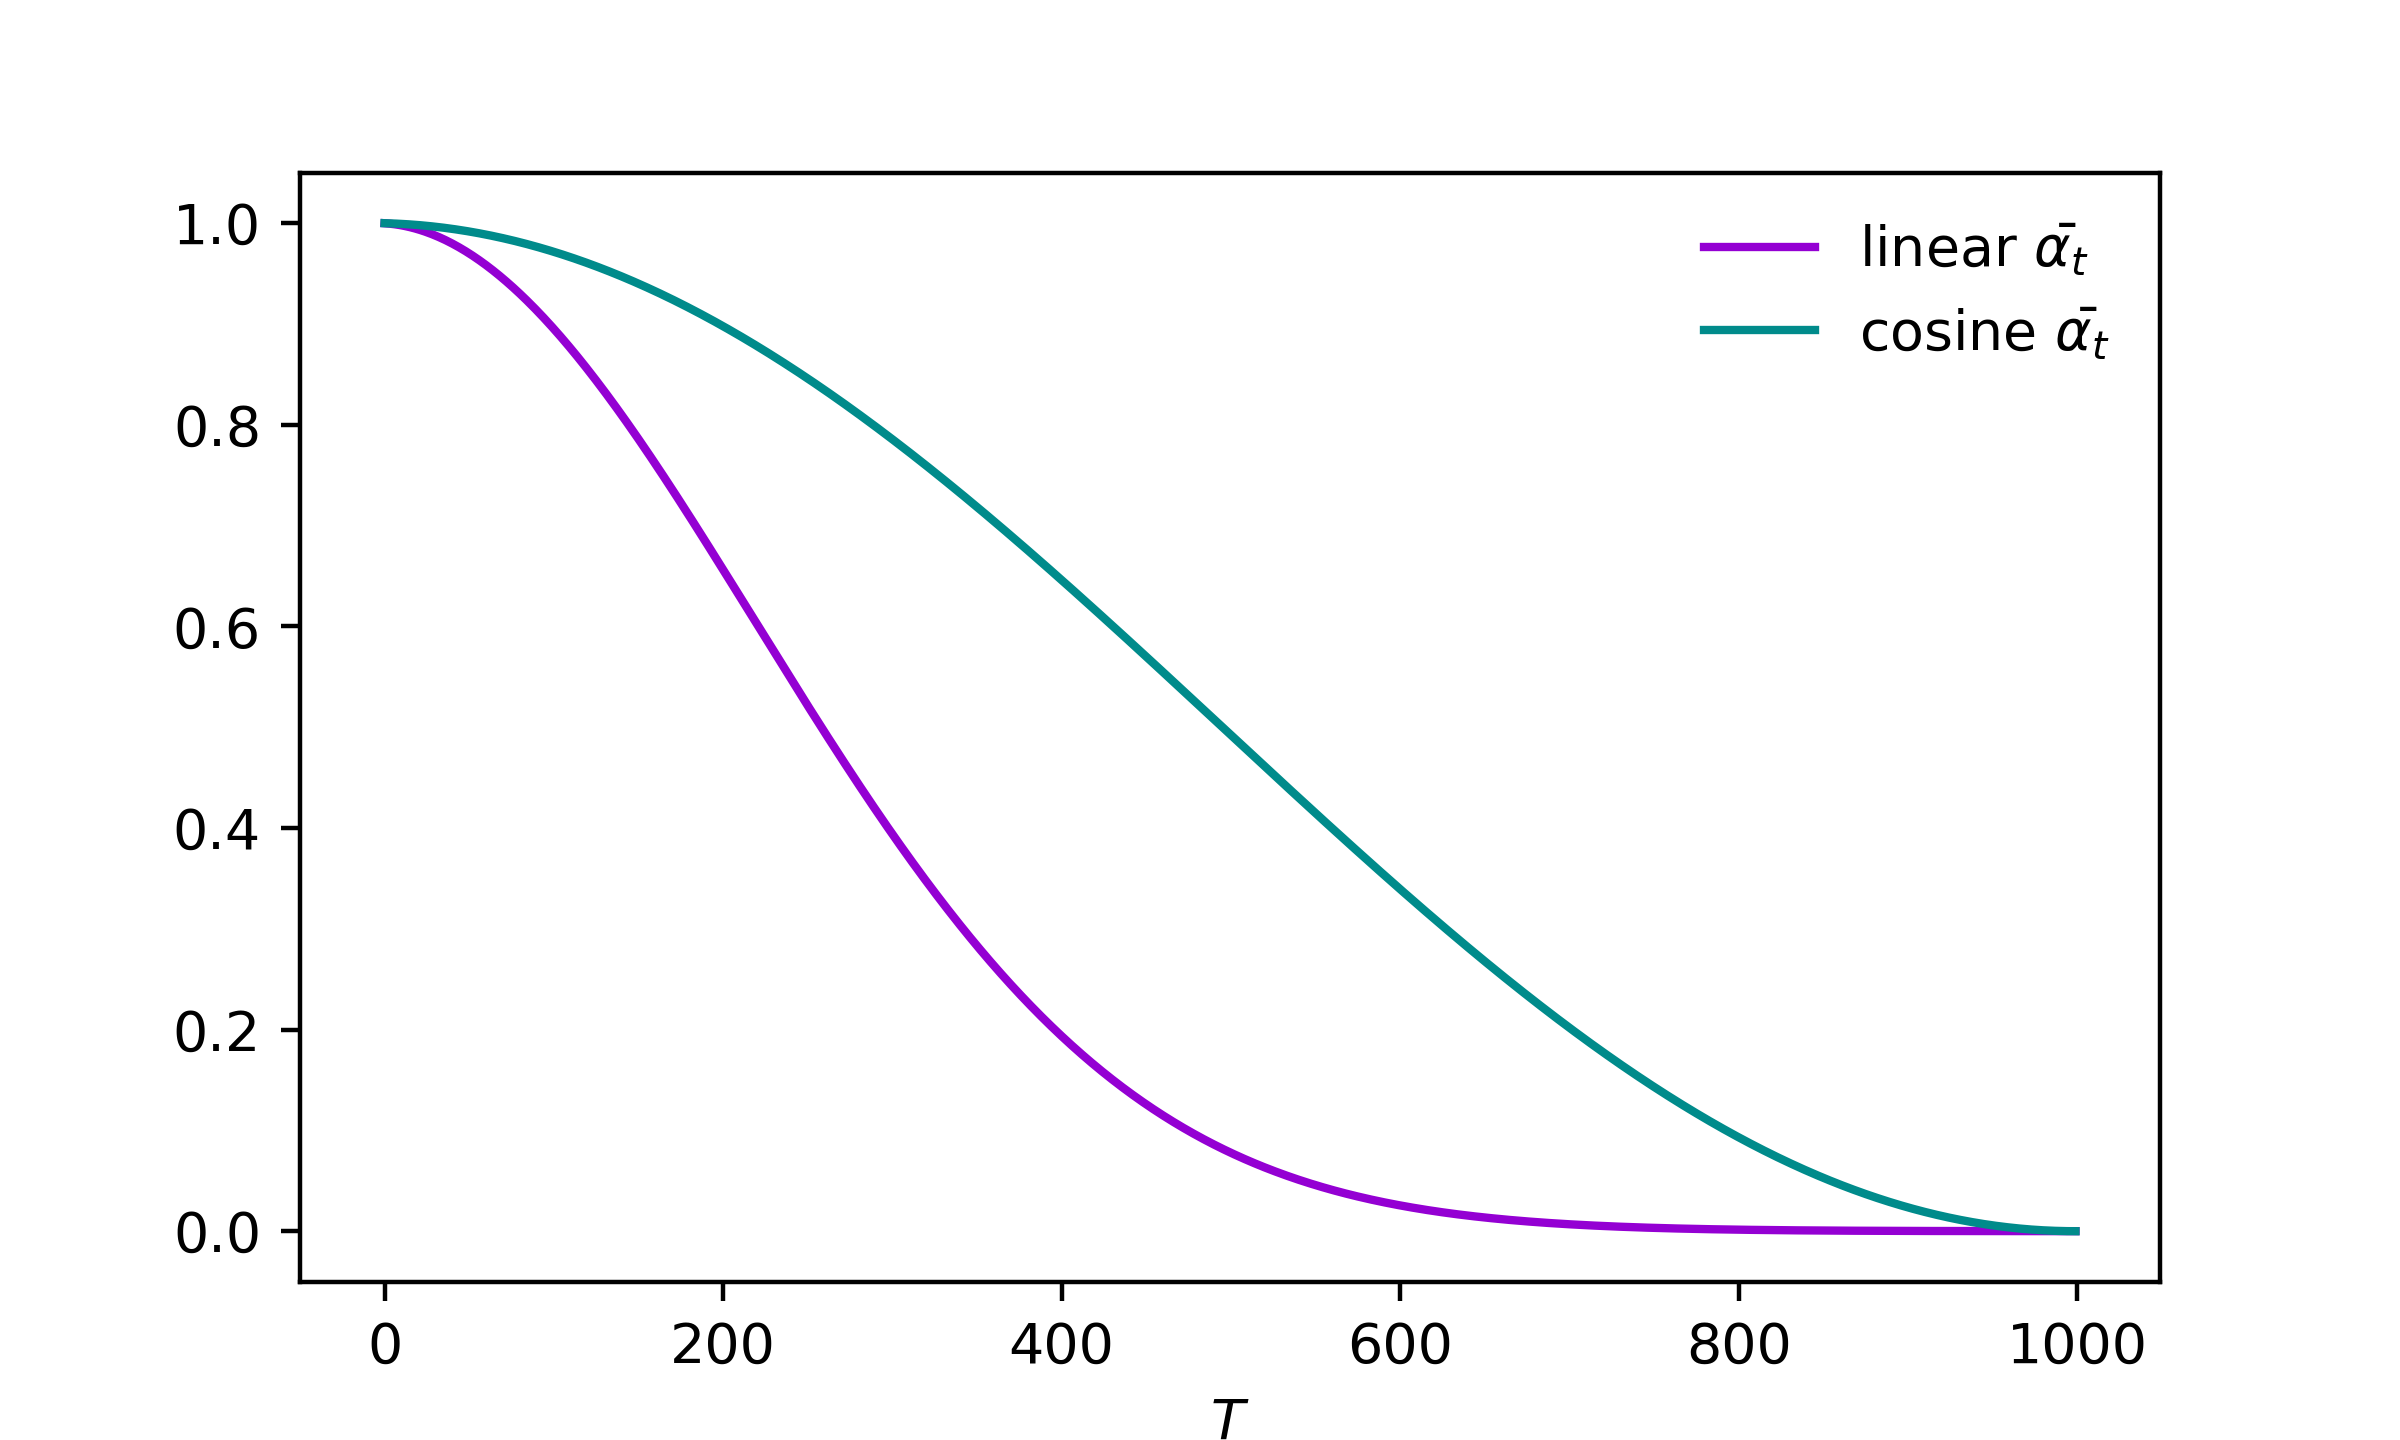
\includegraphics[scale=0.85]{ch2-diffusion-models/ddpm-linear-cosine-scheduler.png}
    \captionsetup{width=\textwidth} % set the width of the caption
    \caption{\textbf{Linear vs. Cosine scheduler} introduce in \cite{nichol2021improved}. Destroying the input structure smoothly is beneficial (regard what?) over using a simple linear scheduler \ca{esta figura suma realmente?}.}
    \label{fig:ddpm-linear-vs-cosine-scheduler}
  \end{figure}

Regarding the variance scheduler, the same work found that the linear scheduler implemented in the DDPM paper was suboptimal because destroying the image very early in the backward chain left a lot of intermediate states redundant. Instead, a cosine scheduler was proposed, which gradually destroys the image structure, providing further informative steps to the denoiser as it shown in Figure~\ref{fig:ddpm-linear-vs-cosine-scheduler}. \\

Notably, the work of \cite{rombach2022highresolution} in improving the model architecture and the training process to scale the resolution.

\subsection{Denoising Diffusion Implicit Models}

The work of \cite{song2020denoising} introduces the Denoising Diffusion Implicit Models (DDIM) that are a score-based model that uses the denoising process to estimate the likelihood of the data. The main difference between DDIM and DDPM is that the former doesn't require a Markovian chain of states to estimate the likelihood. Instead, it uses the denoising process to estimate the likelihood of the data.\\

\begin{equation}\label{eqn:ddim-likelihood}
    x_{t-1} = 
    \sqrt{\alpha_{t-1}}\underbrace{\bigg(\frac{x_{t}-\sqrt{1-\alpha_{t}}\epsilon_{\theta}^{(t)}(x_{t})}{\sqrt{\alpha_{t}}}\bigg)}_{\text{``predicted $x_{0}$''}} 
    + \underbrace{\sqrt{1-\alpha_{t-1} - \sigma^2_{t}}~\cdot~\epsilon_{\theta}^{(t)}(x_{t})}_{\text{``direction pointing to $x_{t}$''}}
    + \underbrace{\sigma_{t}\epsilon_{t}}_{\text{random noise}}
\end{equation}

Esta subsección debe cumplir lo siguiente:

\begin{enumerate}
    \item Explicar los componentes de la ecuación de arriba.
    \item Explicar conexión de la ecuación de arriba con el modelo original DDPM.
    \item Explicar como termino sampleando en menos pasos.
    \item Crear un diagrama donde a la izquierda aparezca una imagen input, al medio el ruido estimado inicial, a la derecha la transformación con
manipulación. Basado en tutorial de Jonatthan Whitakker.
    \item Explicar la utilidad de predecir $\mathrm{x}_{0}$ con el término
    propuesto en DDIM para usarlo con clasificadores no entrenados en ruido, i.e. universal guidance.
\end{enumerate}

\ca{TODO: se puede agregar mini experimentoo con cara de Pedro Pascal. Invertir imagen y luego reconstruirla o pasarla por el proceso de difusión. Siguiente iteración, realizar lo mismo pero con stable diffusion...}


\subsection{Latent Diffusion Models}

XYZ

\section{Neural Net Architecture}

Theoretically, the model with learnable parameters used in the backward process could be anything. However, highly-dimensional data such as images, requires flexible functions that neural networks can handle properly, but not with carefully choose the proper architecture as most Deep Learning implementations. We will briefly discuss the most typical components used within the framework of diffusion models...\\

\begin{itemize}
    \item U-Net
    \item ResNet blocks
    \item Skip connections
    \item Attention blocks
    \item Adaptive group normalization (*)
    \item BigGAN residual block
\end{itemize}


\section{Summary}

In summary, a typical diffusion model framework can be implemented as follows:\\

A \textbf{forward process} that consists of a Markovian chain of states $\{\mathbf{x}\}_{0:T}$ that takes the original image $\mathbf{x}_0$ and iteratively adds noise until getting isotropic Gaussian noise $\mathbf{x}_{T}$. \\

In the reverse, or \textbf{backward process}, a model learns how to gradually remove the noise to recover the data structure. Most implementations model this denoising endeavour using some U-net neural network architecture with attention modules. \\

The model can predict the noisy image directly or indirectly via predicting the noise and then substracting. \ca{\textbf{Agregar:} basicamente que con esa predicción se trata de hacer la estimación con mejor error posible al verdadero ruido, asi se realiza el denoising.}\\

The noise used to destroy the structure in data is carefully handled by a deterministic function called \textbf{noise scheduler}. It determines the variance schedule, $\beta_{1}, \dots, \beta_{T}$, or the specific amount of noise injected in each timestamp $t$ during the Markovian chain. \\

A sequence of intermediate states provides a detailed roadmap to destroy the observation and a trace for the model $p_{\theta}$ to recover the input structure. Therefore, the forward Markovian process acts as a self-supervised generator of labels \ca{providing the noise as a label?}.\\

\ca{\textbf{Agregar:} un parrafo sobre la inferencia y que luego se utiliza simplemente un sampling de la normal y el backward process para obtener nuevas
muestras}.\\

\ca{Será necesario esto acá?}. Initially, the intermediate steps have the exact dimensions of the image. Still, in state of the art implementations, instead of performing the above framework in the pixel space, it is implemented in a latent space. Every intermediate step is a latent representation of the image, represented by a variationoal autencoder, and the model learns to predict the next latent state, reducing significantly the dimensions in which the diffusoin process operate.\ 